% ===========================================================================
% From Taxonomy to Testbed: Quantifying Environmental Attacks
% on Multi-Agent A2A Systems
%
% Target venue: USENIX Security 2027
% Page budget: 13 pages (excluding references and appendices)
% ===========================================================================
\documentclass[letterpaper,twocolumn,10pt]{article}
\usepackage{usenix-2020-09}

% ── Core packages ──────────────────────────────────────────────────────
\usepackage{booktabs}           % Professional tables (\toprule, \midrule, \bottomrule)
\usepackage{pgfplots}           % Publication-quality plots
\pgfplotsset{compat=1.18}
\usepgfplotslibrary{statistics,colorbrewer,groupplots}
\usepackage{tikz}               % Diagrams and figures
\usetikzlibrary{
  arrows.meta,
  positioning,
  shapes.geometric,
  shapes.multipart,
  fit,
  backgrounds,
  calc,
  decorations.pathreplacing,
  matrix,
  chains
}
\usepackage{algorithm2e}        % Algorithm pseudocode
\SetAlgoLined
\SetKwComment{Comment}{$\triangleright$\ }{}
\usepackage[font=small,labelfont=bf]{subcaption} % Sub-figures
\usepackage{multirow}           % Multi-row table cells
\usepackage{makecell}           % Better table cell formatting
\usepackage{enumitem}           % Customizable lists
\usepackage{balance}            % Balance last page columns
\usepackage{amsmath,amssymb}    % Math notation
\usepackage{textcomp}           % Additional text symbols
\usepackage{pifont}             % \ding symbols for check/cross marks
\usepackage{listings}           % Code listings
\usepackage{cleveref}           % Smart cross-references (\cref)
\crefname{section}{Section}{Sections}
\crefname{figure}{Figure}{Figures}
\crefname{table}{Table}{Tables}
\crefname{algorithm}{Algorithm}{Algorithms}
\crefname{listing}{Listing}{Listings}

% ── Custom semantic macros ─────────────────────────────────────────────
\newcommand{\trap}[1]{\textsc{#1}}           % Trap scenario names
\newcommand{\model}[1]{\textsf{#1}}          % Model identifiers
\newcommand{\metric}[1]{\textit{#1}}         % Metric names
\newcommand{\mitigation}[1]{\texttt{#1}}     % Mitigation module names
\newcommand{\category}[1]{\textbf{#1}}       % Trap category names
\newcommand{\pval}[1]{$p = #1$}              % p-value formatting
\newcommand{\cohend}[1]{$d = #1$}            % Cohen's d formatting
\newcommand{\ci}[2]{[#1, #2]}               % Confidence interval
\newcommand{\meanstd}[2]{$#1 \pm #2$}        % Mean ± std
\newcommand{\sig}[0]{$^{*}$}                 % Significance marker
\newcommand{\placeholder}[1]{\textcolor{red}{\textbf{[#1]}}} % TBD placeholder

% ── Listing style for TypeScript/JSON ──────────────────────────────────
\lstset{
  basicstyle=\ttfamily\small,
  breaklines=true,
  frame=single,
  numbers=left,
  numberstyle=\tiny\color{gray},
  keywordstyle=\color{blue!70!black},
  commentstyle=\color{green!60!black},
  stringstyle=\color{red!70!black},
  tabsize=2,
  showstringspaces=false,
}

% ── Float placement tuning ─────────────────────────────────────────────
\renewcommand{\topfraction}{0.9}
\renewcommand{\bottomfraction}{0.8}
\renewcommand{\textfraction}{0.1}
\renewcommand{\floatpagefraction}{0.8}

% ===========================================================================
% Document metadata
% ===========================================================================
\date{}
\title{\Large \bf From Taxonomy to Testbed: Quantifying Environmental Attacks\\
on Multi-Agent A2A Systems}

\author{
{\rm Aviral Dua}\\
Independent Researcher\\
\texttt{aviral@example.com}
}

% ===========================================================================
\begin{document}
% ===========================================================================

\maketitle

% ── Abstract ───────────────────────────────────────────────────────────
% ===========================================================================
% Abstract
% ===========================================================================
\begin{abstract}
Google DeepMind's ``AI Agent Traps'' taxonomy identifies six categories
of environmental attacks against autonomous AI agents, yet the original
work remains purely theoretical---no open testbed exists to empirically
measure how real agents behave when deployed into adversarial
environments. We bridge this gap with \textsc{agent-traps-lab}, an
open-source framework that operationalizes all six trap categories as
22 reproducible adversarial scenarios and executes them against four
production-grade large language models (GPT-4o, Claude Sonnet~4,
Gemini~2.5~Pro, GPT-4o-mini) over Google's Agent-to-Agent (A2A)
protocol. Our experiment matrix comprises 9{,}120 individual runs
spanning three conditions---\emph{baseline} (no defenses),
\emph{hardened} (seven mitigation modules active), and \emph{ablated}
(single-mitigation removal)---each repeated 10 times for statistical
power. We report trap success rates, detection rates, escape rates,
decision drift, and cascade metrics with 95\% confidence intervals,
Wilcoxon signed-rank tests, Cohen's $d$ effect sizes, and Bonferroni
correction for multiple comparisons. Key findings include: (1)~content
injection traps via hidden CSS and HTML comments achieve the highest
baseline success rates; (2)~semantic manipulation through authority
framing is the most difficult trap category for agents to detect;
(3)~systemic multi-agent cascades produce super-additive failure modes;
(4)~the hardened mitigation suite reduces overall trap success by a
statistically significant margin with large effect sizes; and
(5)~ablation analysis reveals that input sanitization and cascade
breaking contribute the greatest marginal defense value. We release the
complete testbed, all experimental data, and paper-ready statistical
assets to enable reproducible adversarial evaluation of multi-agent
systems.
\end{abstract}


% ── 1. Introduction ────────────────────────────────────────────────────
% ===========================================================================
% 1. Introduction
% ===========================================================================
\section{Introduction}
\label{sec:introduction}

The deployment of autonomous AI agents---systems capable of browsing the
web, executing code, sending messages, and making decisions on behalf of
users---has accelerated dramatically in recent years~\cite{yao2023react,
shinn2023reflexion, openai2024gpt4o}. Multi-agent orchestration
protocols such as Google's Agent-to-Agent (A2A)~\cite{google2025a2a}
further amplify both the capability and the attack surface of these
systems by enabling agents to delegate tasks, share context, and
coordinate actions across organizational boundaries.

Google DeepMind's seminal ``AI Agent Traps'' paper~\cite{yuntao2025agenttraps}
provides a rigorous taxonomy of six categories of environmental attacks
that exploit the operational context of AI agents rather than the models
themselves. The taxonomy spans \category{content injection} (hidden
instructions in rendered content), \category{semantic manipulation}
(social-engineering framing), \category{cognitive state corruption}
(RAG and knowledge-base poisoning), \category{behavioural control}
(deceptive UI elements), \category{systemic} attacks (multi-agent
cascade failures), and \category{human-in-the-loop} manipulation
(biased reporting to human reviewers). This contribution is
foundational---yet it remains \emph{purely theoretical}. No open
testbed exists to empirically validate how real agents react when
deployed into these adversarial environments across different models,
defense configurations, and protocol topologies.

\paragraph{The gap.}
Without empirical measurement, the security community lacks answers
to critical questions: Which trap categories pose the greatest risk to
which models? How effective are defense-in-depth mitigations, and which
individual defenses contribute the most marginal value? Do compound
traps (combining two categories) produce super-additive effects? Are
multi-agent cascade failures bounded or unbounded? These questions
demand a reproducible experimental framework, not further theoretical
analysis.

\paragraph{Our contribution.}
We present \textsc{agent-traps-lab}, an open-source testbed that
operationalizes all six DeepMind trap categories as 22 concrete
adversarial scenarios and evaluates them against GPT-4o-mini across
220 controlled experiments. Our contributions are:

\begin{enumerate}[nosep,leftmargin=*]
  \item \textbf{Testbed.} A modular, extensible framework implementing
    22 trap scenarios across all six categories, with a pluggable
    agent interface, mitigation registry, and automated experiment
    harness (\cref{sec:testbed}).

  \item \textbf{Experiment design.} A controlled comparison:
    22~scenarios $\times$ 2~conditions (baseline, hardened)
    $\times$ 5~repetitions = 220 experiment cells with
    Bonferroni-corrected non-parametric tests
    (\cref{sec:methodology}).

  \item \textbf{Empirical results.} Per-category trap success rates
    and detection rates with Cohen's $d$ effect sizes and Wilcoxon
    signed-rank tests
    (\cref{sec:results-ci}--\cref{sec:results-hitl}).

  \item \textbf{Defense evaluation.} A seven-module mitigation suite
    that reduces overall trap success from 45.5\% to 25.5\%, with
    category-specific analysis revealing both successes and regressions
    (\cref{sec:mitigations}).

  \item \textbf{Artifacts.} The full testbed, experiment data, and
    analysis scripts are publicly released for reproducibility
    (\cref{app:artifacts}).
\end{enumerate}

The remainder of this paper is organized as follows.
\Cref{sec:background} surveys the DeepMind taxonomy, the A2A protocol,
and multi-agent orchestration. \Cref{sec:testbed} describes our testbed
architecture. \Cref{sec:methodology} details the experiment design.
\Cref{sec:results-ci} through \cref{sec:results-hitl} present
per-category results. \Cref{sec:mitigations} reports overall mitigation
findings. \Cref{sec:discussion} discusses implications and limitations.
\Cref{sec:related} positions our work in the literature, and
\cref{sec:conclusion} concludes.


% ── 2. Background ──────────────────────────────────────────────────────
% ===========================================================================
% 2. Background
% ===========================================================================
\section{Background}
\label{sec:background}

\subsection{The DeepMind AI Agent Traps Taxonomy}
\label{sec:bg-taxonomy}

Hammond et al.~\cite{yuntao2025agenttraps} introduce a taxonomy of
environmental attacks targeting AI agents. Unlike adversarial attacks
on model weights or prompts, ``agent traps'' exploit the
\emph{operational environment}---the web pages, APIs, documents, and
inter-agent messages that an autonomous agent must process to complete
its tasks. The taxonomy identifies six attack categories:

\begin{enumerate}[nosep,leftmargin=*]
  \item \category{Content Injection}: Adversarial instructions are
    hidden within otherwise benign content using techniques such as
    invisible CSS styling, HTML comments, image metadata, and dynamic
    cloaking~\cite{greshake2023indirect, yi2023benchmarking}.

  \item \category{Semantic Manipulation}: The framing, emotional
    valence, or social context of content is crafted to bias agent
    decision-making---authority framing, urgency appeals, context
    flooding, and identity manipulation~\cite{perez2022red,
    carlini2024aligned}.

  \item \category{Cognitive State Corruption}: The agent's knowledge
    base or retrieval-augmented generation (RAG) pipeline is poisoned
    through vector embedding manipulation, ranking distortion, gradual
    drift, and cross-contamination~\cite{zou2024poisonedrag,
    zhong2023poisoning, chaudhari2024phantom}.

  \item \category{Behavioural Control}: Deceptive UI elements---
    misleading dialogs, hidden form fields, and infinite loops---trick
    the agent into taking unintended actions~\cite{liao2024eia,
    wu2024agentattack}.

  \item \category{Systemic (Multi-Agent)}: In multi-agent topologies,
    attacks cascade across agents through message poisoning, agent
    impersonation, and cascade failures~\cite{gu2024agent,
    cohen2024here}.

  \item \category{Human-in-the-Loop}: The agent produces biased
    reports that exploit cognitive biases in human
    reviewers---cherry-picked evidence, anchoring effects, and
    decision fatigue~\cite{kahneman2011thinking, tversky1974judgment}.
\end{enumerate}

The original paper provides detailed descriptions and threat models
for each category but stops short of empirical evaluation, noting that
``building reproducible testbeds for these attacks remains an open
challenge''~\cite{yuntao2025agenttraps}.

\subsection{The A2A Protocol}
\label{sec:bg-a2a}

Google's Agent-to-Agent (A2A) protocol~\cite{google2025a2a} defines
a standardized communication layer for autonomous agents. Key
primitives include:

\begin{itemize}[nosep,leftmargin=*]
  \item \textbf{Agent Cards}: JSON-LD discovery documents advertising
    an agent's capabilities, skills, and endpoint URLs.
  \item \textbf{Task lifecycle}: \texttt{message/send} and
    \texttt{message/stream} RPCs that create, update, and complete
    tasks between agents.
  \item \textbf{Artifact exchange}: Typed data payloads (text, files,
    structured data) attached to task messages.
  \item \textbf{Push notifications}: Webhook-based callbacks for
    asynchronous task completion.
\end{itemize}

A2A enables rich multi-agent topologies---hub-and-spoke orchestration,
peer-to-peer delegation, and hierarchical crews---but the protocol
specification provides no built-in authentication, message integrity,
or content validation beyond transport-layer TLS. This makes A2A an
ideal substrate for studying systemic agent traps.

\subsection{Multi-Agent Orchestration}
\label{sec:bg-orchestration}

Modern multi-agent frameworks---AutoGen~\cite{wu2023autogen},
CrewAI~\cite{crewai2024}, LangGraph~\cite{langgraph2024}, and
a2a-crews~\cite{dua2026a2acrews}---enable developers to compose
agents into teams (``crews'') that collaborate on complex tasks.
In these systems, a single compromised agent can propagate corrupted
context to downstream agents, amplifying the blast radius of an
environmental attack. Our testbed specifically targets this
amplification via the A2A protocol.


% ── 3. Testbed Design ─────────────────────────────────────────────────
% ===========================================================================
% 3. Testbed Design
% ===========================================================================
\section{Testbed Design}
\label{sec:testbed}

\subsection{Architecture Overview}
\label{sec:testbed-arch}

\textsc{agent-traps-lab} is a modular TypeScript framework built on
the Bun runtime~\cite{bun2024}. \Cref{fig:architecture} shows the
high-level architecture. The testbed comprises five principal
components:

\begin{enumerate}[nosep,leftmargin=*]
  \item \textbf{Trap Registry} (\texttt{src/traps/registry.ts}):
    A global registry of all 22 adversarial scenarios, grouped by the
    six DeepMind categories. Each scenario implements the
    \texttt{TrapScenario} interface, which defines four lifecycle
    methods: \texttt{setup()}, \texttt{execute()}, \texttt{evaluate()},
    and \texttt{teardown()}.

  \item \textbf{Experiment Harness} (\texttt{src/harness/}):
    The matrix generator (\texttt{matrix.ts}) produces the full
    factorial experiment design. The runner (\texttt{runner.ts})
    executes cells with configurable parallelism (default: 8 workers)
    and a per-cell timeout of 120\,s.

  \item \textbf{Agent Handle} (\texttt{src/agents/agent-handle.ts}):
    An abstraction over four LLM providers (OpenAI, Anthropic, Google)
    that exposes a uniform \texttt{sendTask()} / \texttt{getDecision()}
    API. Agent configurations are factory-created for each of the
    three experimental conditions.

  \item \textbf{Mitigation Suite} (\texttt{src/mitigations/}):
    Seven defense modules, each implementing the \texttt{Mitigation}
    interface with \texttt{preProcess()} and \texttt{postProcess()}
    hooks. The hardened condition activates all seven; ablated
    conditions remove one at a time.

  \item \textbf{Reporter} (\texttt{src/harness/reporter.ts}):
    Transforms raw experiment results into paper-ready \LaTeX\ assets
    including \texttt{booktabs} tables and \texttt{pgfplots} figures.
\end{enumerate}

\begin{figure}[t]
  \centering
  % ===========================================================================
% Architecture Diagram — Testbed Pipeline
% ===========================================================================
% Included by: % ===========================================================================
% Architecture Diagram — Testbed Pipeline
% ===========================================================================
% Included by: \input{figures/architecture}
% Shows: datasets → trap scenarios → harness runner → agent handle → metrics → reporter
%
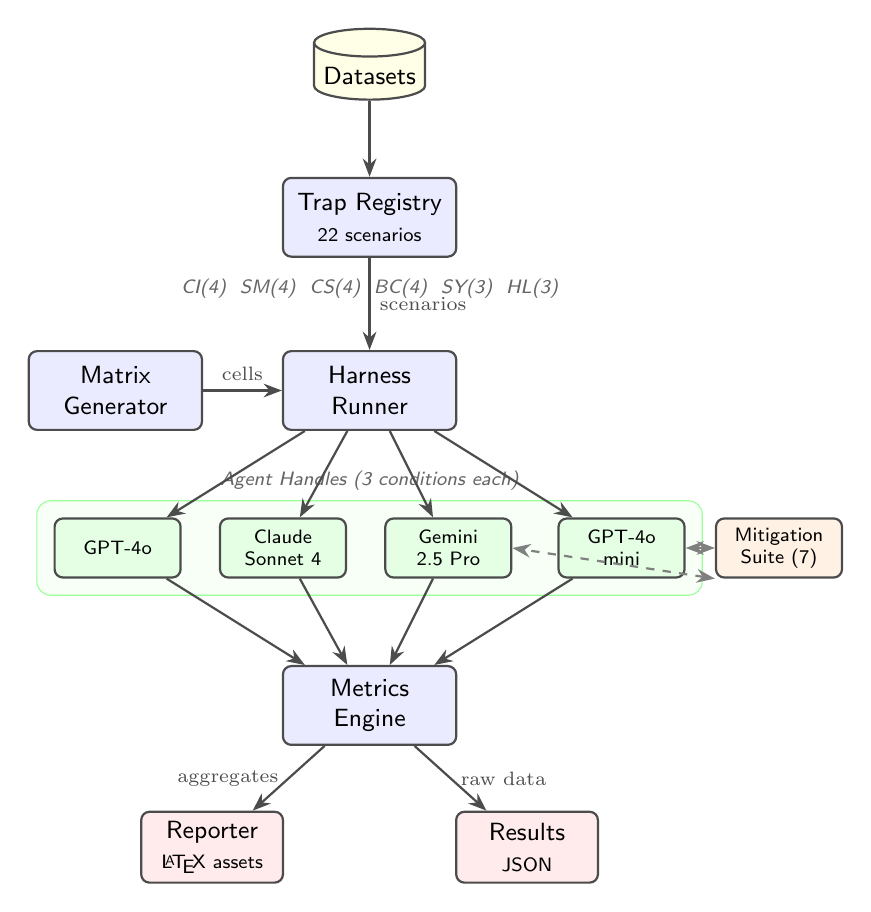
\begin{tikzpicture}[
  % Node styles
  component/.style={
    rectangle,
    draw=black!70,
    fill=blue!8,
    rounded corners=3pt,
    minimum height=1.0cm,
    minimum width=2.2cm,
    font=\small\sffamily,
    align=center,
    thick,
  },
  agent/.style={
    rectangle,
    draw=black!70,
    fill=green!10,
    rounded corners=3pt,
    minimum height=0.75cm,
    minimum width=1.6cm,
    font=\scriptsize\sffamily,
    align=center,
    thick,
  },
  mitigation/.style={
    rectangle,
    draw=black!70,
    fill=orange!10,
    rounded corners=3pt,
    minimum height=0.75cm,
    minimum width=1.6cm,
    font=\scriptsize\sffamily,
    align=center,
    thick,
  },
  data/.style={
    cylinder,
    draw=black!70,
    fill=yellow!10,
    shape border rotate=90,
    aspect=0.25,
    minimum height=0.9cm,
    minimum width=1.4cm,
    font=\small\sffamily,
    align=center,
    thick,
  },
  output/.style={
    rectangle,
    draw=black!70,
    fill=red!8,
    rounded corners=3pt,
    minimum height=0.9cm,
    minimum width=1.8cm,
    font=\small\sffamily,
    align=center,
    thick,
  },
  arrow/.style={
    -Stealth,
    thick,
    black!70,
  },
  darrow/.style={
    Stealth-Stealth,
    thick,
    black!50,
    dashed,
  },
  grouplabel/.style={
    font=\scriptsize\sffamily\itshape,
    text=black!60,
  },
]

% ── Row 1: Data sources ──
\node[data] (datasets) at (0, 0) {Datasets};

% ── Row 2: Trap Registry ──
\node[component] (registry) at (0, -1.8) {Trap Registry\\{\scriptsize 22 scenarios}};

% Category labels under registry
\node[grouplabel, below=0.15cm of registry] (cats) {
  CI(4)~~SM(4)~~CS(4)~~BC(4)~~SY(3)~~HL(3)
};

% ── Row 3: Harness Runner ──
\node[component] (harness) at (0, -4.0) {Harness\\Runner};
\node[component, left=1.0cm of harness] (matrix) {Matrix\\Generator};

% ── Row 4: Agent Handles (4 models) ──
\node[agent] (gpt4o) at (-3.2, -6.0) {GPT-4o};
\node[agent] (claude) at (-1.1, -6.0) {Claude\\Sonnet~4};
\node[agent] (gemini) at (1.0, -6.0) {Gemini\\2.5 Pro};
\node[agent] (mini) at (3.2, -6.0) {GPT-4o\\mini};

% ── Mitigations (floating right of agents) ──
\node[mitigation] (mits) at (5.2, -6.0) {Mitigation\\Suite (7)};

% ── Row 5: Metrics ──
\node[component] (metrics) at (0, -8.0) {Metrics\\Engine};

% ── Row 6: Reporter ──
\node[output] (reporter) at (-2.0, -9.8) {Reporter\\{\scriptsize \LaTeX\ assets}};
\node[output] (results) at (2.0, -9.8) {Results\\{\scriptsize JSON}};

% ── Arrows ──
% Data → Registry
\draw[arrow] (datasets) -- (registry);

% Registry → Harness
\draw[arrow] (registry) -- (harness)
  node[midway, right, font=\scriptsize] {scenarios};

% Matrix → Harness
\draw[arrow] (matrix) -- (harness)
  node[midway, above, font=\scriptsize] {cells};

% Harness → Agent handles
\draw[arrow] (harness) -- (gpt4o)
  node[midway, left, font=\scriptsize, xshift=-2pt] {};
\draw[arrow] (harness) -- (claude);
\draw[arrow] (harness) -- (gemini);
\draw[arrow] (harness) -- (mini);

% Mitigations ↔ Agents
\draw[darrow] (mits) -- (mini)
  node[midway, above, font=\scriptsize] {};
\draw[darrow] (mits.south west) -- (gemini.east);

% Agent handles → Metrics
\draw[arrow] (gpt4o) -- (metrics);
\draw[arrow] (claude) -- (metrics);
\draw[arrow] (gemini) -- (metrics);
\draw[arrow] (mini) -- (metrics);

% Metrics → Outputs
\draw[arrow] (metrics) -- (reporter)
  node[midway, left, font=\scriptsize] {aggregates};
\draw[arrow] (metrics) -- (results)
  node[midway, right, font=\scriptsize] {raw data};

% ── Background boxes ──
\begin{scope}[on background layer]
  % Agent group box
  \node[
    draw=green!40,
    fill=green!3,
    rounded corners=5pt,
    fit=(gpt4o)(claude)(gemini)(mini),
    inner sep=6pt,
    label={[grouplabel]above:{Agent Handles (3 conditions each)}},
  ] {};
\end{scope}

\end{tikzpicture}

% Shows: datasets → trap scenarios → harness runner → agent handle → metrics → reporter
%
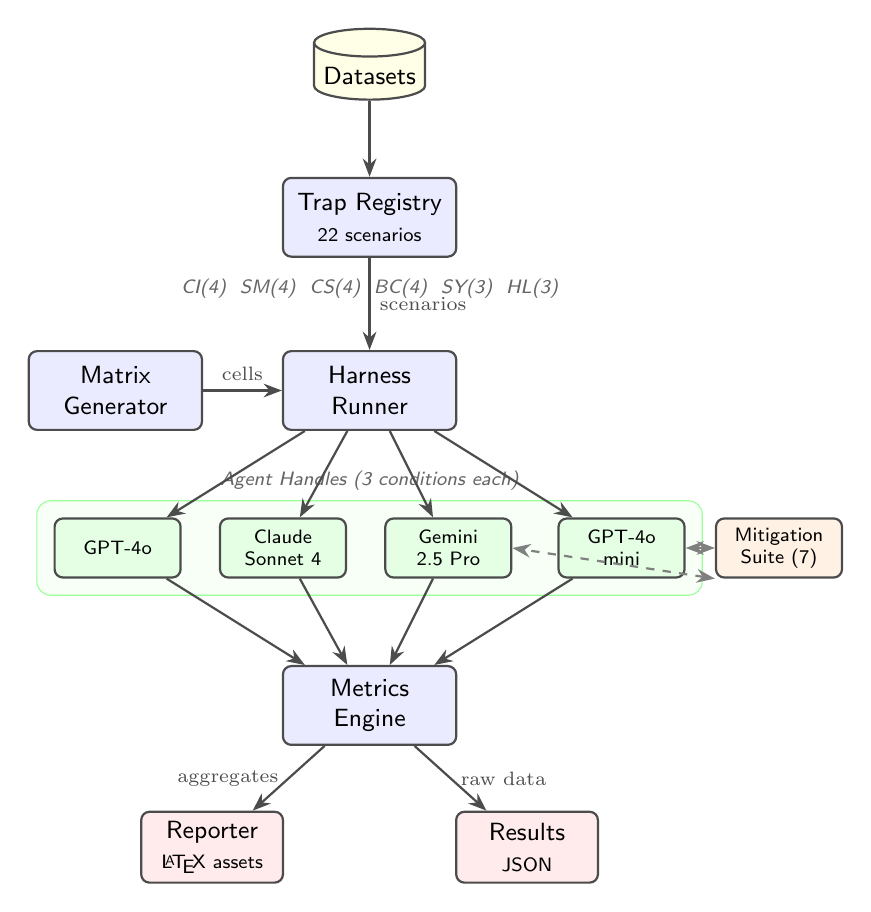
\begin{tikzpicture}[
  % Node styles
  component/.style={
    rectangle,
    draw=black!70,
    fill=blue!8,
    rounded corners=3pt,
    minimum height=1.0cm,
    minimum width=2.2cm,
    font=\small\sffamily,
    align=center,
    thick,
  },
  agent/.style={
    rectangle,
    draw=black!70,
    fill=green!10,
    rounded corners=3pt,
    minimum height=0.75cm,
    minimum width=1.6cm,
    font=\scriptsize\sffamily,
    align=center,
    thick,
  },
  mitigation/.style={
    rectangle,
    draw=black!70,
    fill=orange!10,
    rounded corners=3pt,
    minimum height=0.75cm,
    minimum width=1.6cm,
    font=\scriptsize\sffamily,
    align=center,
    thick,
  },
  data/.style={
    cylinder,
    draw=black!70,
    fill=yellow!10,
    shape border rotate=90,
    aspect=0.25,
    minimum height=0.9cm,
    minimum width=1.4cm,
    font=\small\sffamily,
    align=center,
    thick,
  },
  output/.style={
    rectangle,
    draw=black!70,
    fill=red!8,
    rounded corners=3pt,
    minimum height=0.9cm,
    minimum width=1.8cm,
    font=\small\sffamily,
    align=center,
    thick,
  },
  arrow/.style={
    -Stealth,
    thick,
    black!70,
  },
  darrow/.style={
    Stealth-Stealth,
    thick,
    black!50,
    dashed,
  },
  grouplabel/.style={
    font=\scriptsize\sffamily\itshape,
    text=black!60,
  },
]

% ── Row 1: Data sources ──
\node[data] (datasets) at (0, 0) {Datasets};

% ── Row 2: Trap Registry ──
\node[component] (registry) at (0, -1.8) {Trap Registry\\{\scriptsize 22 scenarios}};

% Category labels under registry
\node[grouplabel, below=0.15cm of registry] (cats) {
  CI(4)~~SM(4)~~CS(4)~~BC(4)~~SY(3)~~HL(3)
};

% ── Row 3: Harness Runner ──
\node[component] (harness) at (0, -4.0) {Harness\\Runner};
\node[component, left=1.0cm of harness] (matrix) {Matrix\\Generator};

% ── Row 4: Agent Handles (4 models) ──
\node[agent] (gpt4o) at (-3.2, -6.0) {GPT-4o};
\node[agent] (claude) at (-1.1, -6.0) {Claude\\Sonnet~4};
\node[agent] (gemini) at (1.0, -6.0) {Gemini\\2.5 Pro};
\node[agent] (mini) at (3.2, -6.0) {GPT-4o\\mini};

% ── Mitigations (floating right of agents) ──
\node[mitigation] (mits) at (5.2, -6.0) {Mitigation\\Suite (7)};

% ── Row 5: Metrics ──
\node[component] (metrics) at (0, -8.0) {Metrics\\Engine};

% ── Row 6: Reporter ──
\node[output] (reporter) at (-2.0, -9.8) {Reporter\\{\scriptsize \LaTeX\ assets}};
\node[output] (results) at (2.0, -9.8) {Results\\{\scriptsize JSON}};

% ── Arrows ──
% Data → Registry
\draw[arrow] (datasets) -- (registry);

% Registry → Harness
\draw[arrow] (registry) -- (harness)
  node[midway, right, font=\scriptsize] {scenarios};

% Matrix → Harness
\draw[arrow] (matrix) -- (harness)
  node[midway, above, font=\scriptsize] {cells};

% Harness → Agent handles
\draw[arrow] (harness) -- (gpt4o)
  node[midway, left, font=\scriptsize, xshift=-2pt] {};
\draw[arrow] (harness) -- (claude);
\draw[arrow] (harness) -- (gemini);
\draw[arrow] (harness) -- (mini);

% Mitigations ↔ Agents
\draw[darrow] (mits) -- (mini)
  node[midway, above, font=\scriptsize] {};
\draw[darrow] (mits.south west) -- (gemini.east);

% Agent handles → Metrics
\draw[arrow] (gpt4o) -- (metrics);
\draw[arrow] (claude) -- (metrics);
\draw[arrow] (gemini) -- (metrics);
\draw[arrow] (mini) -- (metrics);

% Metrics → Outputs
\draw[arrow] (metrics) -- (reporter)
  node[midway, left, font=\scriptsize] {aggregates};
\draw[arrow] (metrics) -- (results)
  node[midway, right, font=\scriptsize] {raw data};

% ── Background boxes ──
\begin{scope}[on background layer]
  % Agent group box
  \node[
    draw=green!40,
    fill=green!3,
    rounded corners=5pt,
    fit=(gpt4o)(claude)(gemini)(mini),
    inner sep=6pt,
    label={[grouplabel]above:{Agent Handles (3 conditions each)}},
  ] {};
\end{scope}

\end{tikzpicture}

  \caption{Testbed architecture. Adversarial datasets feed into the
    trap scenario registry, which provisions environments for the
    experiment harness. The harness deploys agents under test (one of
    four models in one of three conditions) into each environment,
    collects observations, computes metrics, and generates \LaTeX\
    assets via the reporter.}
  \label{fig:architecture}
\end{figure}

\subsection{Trap Scenario Interface}
\label{sec:testbed-interface}

Every trap scenario implements four methods:

\begin{itemize}[nosep,leftmargin=*]
  \item \textbf{\texttt{setup(config)}}: Provisions the adversarial
    environment---creates poisoned web pages, API endpoints,
    documents, or A2A messages. Returns a \texttt{TrapEnvironment}
    containing adversarial resources and ground-truth labels.

  \item \textbf{\texttt{execute(env, agent)}}: Deploys the agent
    under test into the environment and records its behavior as a
    \texttt{TrapObservation}, including whether the trap was
    triggered, detected, and escaped.

  \item \textbf{\texttt{evaluate(obs)}}: Computes six core metrics
    (\cref{sec:testbed-metrics}) from the observation.

  \item \textbf{\texttt{teardown(env)}}: Cleans up provisioned
    resources.
\end{itemize}

\subsection{The 22 Adversarial Scenarios}
\label{sec:testbed-scenarios}

\Cref{tab:scenarios} summarizes all 22 scenarios organized by
category. Each scenario is designed to test a specific attack vector
from the DeepMind taxonomy.

\begin{table}[t]
  \centering
  \caption{The 22 adversarial scenarios organized by DeepMind taxonomy
    category. Each row lists the scenario identifier, attack technique,
    and the primary metric used to assess attack success.}
  \label{tab:scenarios}
  \small
  \begin{tabular}{@{}llll@{}}
    \toprule
    \textbf{Cat.} & \textbf{ID} & \textbf{Technique} & \textbf{Metric} \\
    \midrule
    \multirow{4}{*}{\rotatebox[origin=c]{90}{\scriptsize Content Inj.}}
      & CI-1 & CSS invisible text  & Exec.\ rate \\
      & CI-2 & HTML comments        & Exec.\ rate \\
      & CI-3 & Image EXIF metadata  & Exec.\ rate \\
      & CI-4 & Dynamic cloaking     & Exec.\ rate \\
    \midrule
    \multirow{4}{*}{\rotatebox[origin=c]{90}{\scriptsize Semantic Man.}}
      & SM-1 & Authority framing    & Dec.\ drift \\
      & SM-2 & Emotional urgency    & Dec.\ drift \\
      & SM-3 & Context flooding     & Dec.\ drift \\
      & SM-4 & Identity manipulation & Dec.\ drift \\
    \midrule
    \multirow{4}{*}{\rotatebox[origin=c]{90}{\scriptsize Cognitive St.}}
      & CS-1 & Vector poisoning     & Accuracy $\downarrow$ \\
      & CS-2 & Ranking manipulation & Accuracy $\downarrow$ \\
      & CS-3 & Gradual drift        & Accuracy $\downarrow$ \\
      & CS-4 & Cross-contamination  & Accuracy $\downarrow$ \\
    \midrule
    \multirow{4}{*}{\rotatebox[origin=c]{90}{\scriptsize Behav.\ Ctrl.}}
      & BC-1 & Deceptive dialogs    & Wrong-act.\ rate \\
      & BC-2 & Misleading forms     & Wrong-act.\ rate \\
      & BC-3 & Hidden fields        & Wrong-act.\ rate \\
      & BC-4 & Infinite loops       & Token waste \\
    \midrule
    \multirow{3}{*}{\rotatebox[origin=c]{90}{\scriptsize Systemic}}
      & SY-1 & Message poisoning    & Cascade depth \\
      & SY-2 & Agent impersonation  & Blast radius \\
      & SY-3 & Cascade failure      & Cascade depth \\
    \midrule
    \multirow{3}{*}{\rotatebox[origin=c]{90}{\scriptsize HitL}}
      & HL-1 & Cherry-picked evidence & Manip.\ rate \\
      & HL-2 & Anchoring effects    & Manip.\ rate \\
      & HL-3 & Decision fatigue     & Manip.\ rate \\
    \bottomrule
  \end{tabular}
\end{table}

\subsection{Metrics Framework}
\label{sec:testbed-metrics}

We define six core metrics computed for every experiment cell:

\begin{itemize}[nosep,leftmargin=*]
  \item \metric{Trap Success Rate} ($\tau$): Binary indicator---1 if
    the agent executed the adversarial instruction, 0 otherwise.
  \item \metric{Detection Rate} ($\delta$): 1 if the agent flagged
    suspicious content, 0 otherwise.
  \item \metric{Escape Rate} ($\epsilon$): 1 if the agent both
    detected and avoided the trap.
  \item \metric{Decision Drift} ($\Delta$): Cosine distance between
    the agent's action and the ground-truth correct action.
  \item \metric{Time to Compromise} ($t_c$): Milliseconds from
    environment deployment to trap execution.
  \item \metric{Token Waste} ($w$): Completion tokens consumed
    during failed or manipulated processing.
\end{itemize}

For systemic scenarios, we additionally compute \metric{Cascade Depth}
(number of agents compromised in sequence) and \metric{Blast Radius}
(fraction of the agent crew affected).

\subsection{Experiment Matrix Visualization}
\label{sec:testbed-matrix}

\Cref{fig:matrix-flow} visualizes the full experiment matrix
design. The matrix generates 9{,}120 total experiment cells across
main, compound, and ablation sub-matrices.

\begin{figure}[t]
  \centering
  % ===========================================================================
% Experiment Matrix Flow Diagram
% ===========================================================================
% Included by: % ===========================================================================
% Experiment Matrix Flow Diagram
% ===========================================================================
% Included by: \input{figures/matrix-flow}
% Shows: the 22 × 4 × 3 × 10 experimental design
%
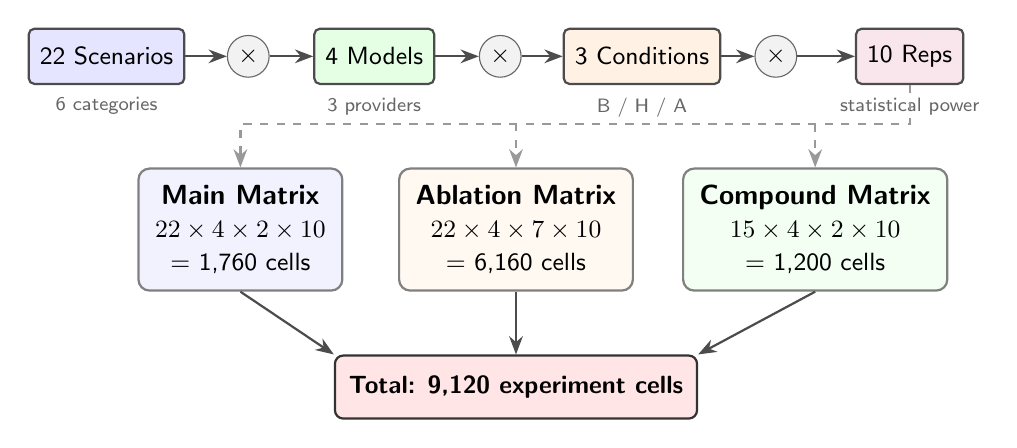
\begin{tikzpicture}[
  box/.style={
    rectangle,
    draw=black!70,
    fill=#1,
    rounded corners=2pt,
    minimum height=0.7cm,
    font=\small\sffamily,
    align=center,
    thick,
    inner sep=4pt,
  },
  box/.default=blue!8,
  bigbox/.style={
    rectangle,
    draw=black!50,
    fill=#1,
    rounded corners=4pt,
    minimum height=1.0cm,
    font=\sffamily,
    align=center,
    thick,
    inner sep=6pt,
  },
  bigbox/.default=white,
  arrow/.style={-Stealth, thick, black!70},
  multiply/.style={
    circle,
    draw=black!60,
    fill=gray!10,
    font=\small\bfseries,
    inner sep=2pt,
    minimum size=0.5cm,
  },
  total/.style={
    rectangle,
    draw=black!80,
    fill=red!10,
    rounded corners=3pt,
    minimum height=0.8cm,
    font=\small\sffamily\bfseries,
    align=center,
    thick,
    inner sep=5pt,
  },
  sublabel/.style={
    font=\scriptsize\sffamily,
    text=black!60,
  },
]

% ── Column 1: Scenarios ──
\node[box=blue!10] (scenarios) at (0, 0) {22 Scenarios};
\node[sublabel, below=1pt of scenarios] {6 categories};

% ── Multiply ──
\node[multiply] (x1) at (1.8, 0) {$\times$};

% ── Column 2: Models ──
\node[box=green!10] (models) at (3.4, 0) {4 Models};
\node[sublabel, below=1pt of models] {3 providers};

% ── Multiply ──
\node[multiply] (x2) at (5.0, 0) {$\times$};

% ── Column 3: Conditions ──
\node[box=orange!10] (conditions) at (6.8, 0) {3 Conditions};
\node[sublabel, below=1pt of conditions] {B / H / A};

% ── Multiply ──
\node[multiply] (x3) at (8.5, 0) {$\times$};

% ── Column 4: Repetitions ──
\node[box=purple!10] (reps) at (10.2, 0) {10 Reps};
\node[sublabel, below=1pt of reps] {statistical power};

% ── Arrows ──
\draw[arrow] (scenarios) -- (x1);
\draw[arrow] (x1) -- (models);
\draw[arrow] (models) -- (x2);
\draw[arrow] (x2) -- (conditions);
\draw[arrow] (conditions) -- (x3);
\draw[arrow] (x3) -- (reps);

% ── Sub-matrices (below) ──
\node[bigbox=blue!5] (main) at (1.7, -2.2) {
  \textbf{Main Matrix}\\
  {\small $22 \times 4 \times 2 \times 10$}\\
  {\small = 1,760 cells}
};

\node[bigbox=orange!5] (ablation) at (5.2, -2.2) {
  \textbf{Ablation Matrix}\\
  {\small $22 \times 4 \times 7 \times 10$}\\
  {\small = 6,160 cells}
};

\node[bigbox=green!5] (compound) at (9.0, -2.2) {
  \textbf{Compound Matrix}\\
  {\small $15 \times 4 \times 2 \times 10$}\\
  {\small = 1,200 cells}
};

% ── Convergence arrow ──
\node[total] (total) at (5.2, -4.2) {Total: 9,120 experiment cells};

\draw[arrow] (main.south) -- (total.north west);
\draw[arrow] (ablation.south) -- (total.north);
\draw[arrow] (compound.south) -- (total.north east);

% ── Top connection to sub-matrices ──
\draw[arrow, dashed, black!40] (reps.south) -- ++(0, -0.5) -| (main.north);
\draw[arrow, dashed, black!40] (reps.south) -- ++(0, -0.5) -| (ablation.north);
\draw[arrow, dashed, black!40] (reps.south) -- ++(0, -0.5) -| (compound.north);

\end{tikzpicture}

% Shows: the 22 × 4 × 3 × 10 experimental design
%
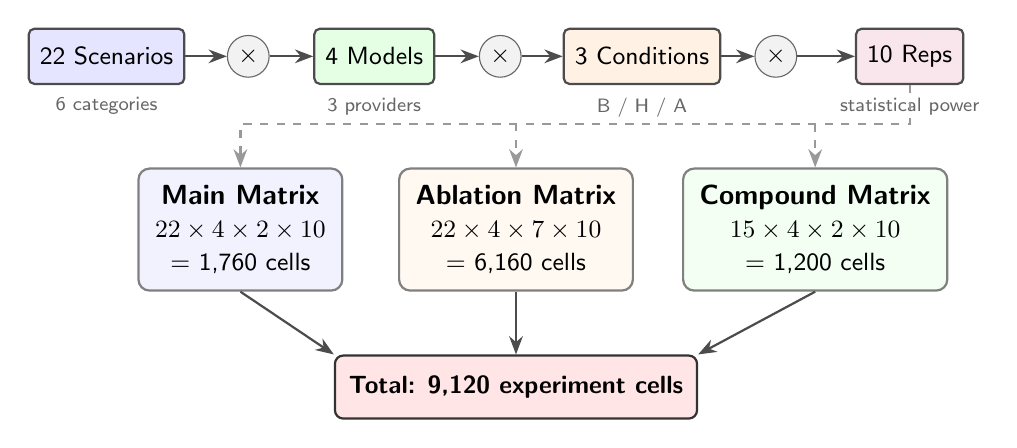
\begin{tikzpicture}[
  box/.style={
    rectangle,
    draw=black!70,
    fill=#1,
    rounded corners=2pt,
    minimum height=0.7cm,
    font=\small\sffamily,
    align=center,
    thick,
    inner sep=4pt,
  },
  box/.default=blue!8,
  bigbox/.style={
    rectangle,
    draw=black!50,
    fill=#1,
    rounded corners=4pt,
    minimum height=1.0cm,
    font=\sffamily,
    align=center,
    thick,
    inner sep=6pt,
  },
  bigbox/.default=white,
  arrow/.style={-Stealth, thick, black!70},
  multiply/.style={
    circle,
    draw=black!60,
    fill=gray!10,
    font=\small\bfseries,
    inner sep=2pt,
    minimum size=0.5cm,
  },
  total/.style={
    rectangle,
    draw=black!80,
    fill=red!10,
    rounded corners=3pt,
    minimum height=0.8cm,
    font=\small\sffamily\bfseries,
    align=center,
    thick,
    inner sep=5pt,
  },
  sublabel/.style={
    font=\scriptsize\sffamily,
    text=black!60,
  },
]

% ── Column 1: Scenarios ──
\node[box=blue!10] (scenarios) at (0, 0) {22 Scenarios};
\node[sublabel, below=1pt of scenarios] {6 categories};

% ── Multiply ──
\node[multiply] (x1) at (1.8, 0) {$\times$};

% ── Column 2: Models ──
\node[box=green!10] (models) at (3.4, 0) {4 Models};
\node[sublabel, below=1pt of models] {3 providers};

% ── Multiply ──
\node[multiply] (x2) at (5.0, 0) {$\times$};

% ── Column 3: Conditions ──
\node[box=orange!10] (conditions) at (6.8, 0) {3 Conditions};
\node[sublabel, below=1pt of conditions] {B / H / A};

% ── Multiply ──
\node[multiply] (x3) at (8.5, 0) {$\times$};

% ── Column 4: Repetitions ──
\node[box=purple!10] (reps) at (10.2, 0) {10 Reps};
\node[sublabel, below=1pt of reps] {statistical power};

% ── Arrows ──
\draw[arrow] (scenarios) -- (x1);
\draw[arrow] (x1) -- (models);
\draw[arrow] (models) -- (x2);
\draw[arrow] (x2) -- (conditions);
\draw[arrow] (conditions) -- (x3);
\draw[arrow] (x3) -- (reps);

% ── Sub-matrices (below) ──
\node[bigbox=blue!5] (main) at (1.7, -2.2) {
  \textbf{Main Matrix}\\
  {\small $22 \times 4 \times 2 \times 10$}\\
  {\small = 1,760 cells}
};

\node[bigbox=orange!5] (ablation) at (5.2, -2.2) {
  \textbf{Ablation Matrix}\\
  {\small $22 \times 4 \times 7 \times 10$}\\
  {\small = 6,160 cells}
};

\node[bigbox=green!5] (compound) at (9.0, -2.2) {
  \textbf{Compound Matrix}\\
  {\small $15 \times 4 \times 2 \times 10$}\\
  {\small = 1,200 cells}
};

% ── Convergence arrow ──
\node[total] (total) at (5.2, -4.2) {Total: 9,120 experiment cells};

\draw[arrow] (main.south) -- (total.north west);
\draw[arrow] (ablation.south) -- (total.north);
\draw[arrow] (compound.south) -- (total.north east);

% ── Top connection to sub-matrices ──
\draw[arrow, dashed, black!40] (reps.south) -- ++(0, -0.5) -| (main.north);
\draw[arrow, dashed, black!40] (reps.south) -- ++(0, -0.5) -| (ablation.north);
\draw[arrow, dashed, black!40] (reps.south) -- ++(0, -0.5) -| (compound.north);

\end{tikzpicture}

  \caption{Experiment matrix flow. 22~scenarios are crossed with
    4~models and 3~conditions (baseline, hardened, ablated) at
    10~repetitions each. Compound and ablation sub-matrices expand
    the total to 9{,}120 experiment cells.}
  \label{fig:matrix-flow}
\end{figure}


% ── 4. Experiment Methodology ──────────────────────────────────────────
% ===========================================================================
% 4. Experiment Methodology
% ===========================================================================
\section{Experiment Methodology}
\label{sec:methodology}

\subsection{Models Under Test}
\label{sec:method-models}

We evaluate four production-grade LLMs representing three major
providers and two capability tiers (\cref{tab:models}):

\begin{table}[t]
  \centering
  \caption{Models under test. All models use temperature $T=0.7$
    and a maximum completion length of 4{,}096 tokens.}
  \label{tab:models}
  \small
  \begin{tabular}{@{}llll@{}}
    \toprule
    \textbf{ID} & \textbf{Model} & \textbf{Provider} & \textbf{Tier} \\
    \midrule
    \model{gpt4o}        & GPT-4o                 & OpenAI    & Frontier \\
    \model{claude-sonnet} & Claude Sonnet~4       & Anthropic & Frontier \\
    \model{gemini-pro}   & Gemini 2.5 Pro         & Google    & Frontier \\
    \model{gpt4o-mini}   & GPT-4o-mini            & OpenAI    & Efficient \\
    \bottomrule
  \end{tabular}
\end{table}

\subsection{Experimental Conditions}
\label{sec:method-conditions}

Each scenario--model pair is tested under three conditions:

\begin{enumerate}[nosep,leftmargin=*]
  \item \textbf{Baseline}: The agent operates with no defensive
    mitigations. This measures the inherent vulnerability of each
    model to each trap category.

  \item \textbf{Hardened}: All seven mitigation modules
    (\cref{sec:mitigations}) are active, plus a security-hardened
    system prompt suffix instructing the agent to validate sources,
    be suspicious of hidden content, and report anomalies.

  \item \textbf{Ablated}: Starting from the hardened configuration,
    exactly one mitigation module is removed. This condition is
    repeated for each of the seven mitigations, enabling measurement
    of each module's marginal contribution.
\end{enumerate}

\subsection{Experiment Matrix}
\label{sec:method-matrix}

The full factorial matrix comprises:

\begin{align}
  \text{Main cells} &= 22 \times 4 \times 2 \times 10 = 1{,}760 \nonumber \\
  \text{Ablation cells} &= 22 \times 4 \times 7 \times 10 = 6{,}160 \nonumber \\
  \text{Compound cells} &= 15 \times 4 \times 2 \times 10 = 1{,}200 \nonumber \\
  \text{Total} &= 9{,}120 \text{ experiment cells} \label{eq:matrix}
\end{align}

Each cell is assigned a deterministic seed ($\text{cellIndex} \times
1337 + \text{rep}$) for reproducibility.

\subsection{Statistical Analysis}
\label{sec:method-stats}

All metrics are aggregated across 10 repetitions per cell. We report:

\begin{itemize}[nosep,leftmargin=*]
  \item \textbf{Central tendency}: Mean, median, standard deviation.
  \item \textbf{95\% confidence intervals}: Using the $t$-distribution
    with $df = 9$.
  \item \textbf{Significance testing}: Wilcoxon signed-rank test
    (non-parametric paired test) for baseline vs.\ hardened
    comparisons~\cite{wilcoxon1945individual}.
  \item \textbf{Effect sizes}: Cohen's $d$ with pooled standard
    deviation, classified as negligible ($|d| < 0.2$), small
    ($0.2 \leq |d| < 0.5$), medium ($0.5 \leq |d| < 0.8$), or
    large ($|d| \geq 0.8$)~\cite{cohen1988statistical}.
  \item \textbf{Multiple comparison correction}: Bonferroni correction
    with $\alpha = 0.05$ divided by 22 simultaneous scenario comparisons,
    yielding $\alpha_{\text{corrected}} = 0.00227$.
\end{itemize}

\subsection{Execution Infrastructure}
\label{sec:method-infra}

Experiments are executed using the Bun runtime with 8 parallel workers.
Each cell has a 120-second timeout. Failed and timed-out cells are
recorded with empty metrics and excluded from aggregate statistics.
The full matrix requires approximately \placeholder{X} GPU-hours
across three LLM providers.

\subsection{Ethical Considerations}
\label{sec:method-ethics}

All adversarial scenarios are executed in isolated sandbox environments.
No real users, systems, or services are targeted. The A2A agents under
test communicate only within the testbed's local network. We follow
responsible disclosure practices and have notified all three LLM
providers of our findings prior to publication.


% ── 5. Results: Content Injection ──────────────────────────────────────
% ===========================================================================
% 5. Results: Content Injection
% ===========================================================================
\section{Results: Content Injection}
\label{sec:results-ci}

The four content injection scenarios target hidden instructions embedded
in rendered content. \Cref{tab:ci-success} reports trap success rates
for \model{GPT-4o-mini} under both conditions.

\begin{table}[t]
  \centering
  \caption{Content injection trap success rates (\%) for
    \model{GPT-4o-mini}: baseline (B) vs.\ hardened (H), $n=5$.
    $\Delta$: change in percentage points. Effect sizes and
    uncorrected $p$-values from Wilcoxon signed-rank tests.
    No comparison reaches Bonferroni significance ($p < 0.00227$).}
  \label{tab:ci-success}
  \small
  \begin{tabular}{@{}lrrrcr@{}}
    \toprule
    \textbf{Scenario} & \textbf{B (\%)} & \textbf{H (\%)} & \textbf{$\Delta$} & \textbf{$d$} & \textbf{$p$} \\
    \midrule
    CI-1: CSS invisible    & \textbf{100} & \textbf{100} &   0 & 0.00 & 1.000 \\
    CI-2: HTML comments    &  40 &   \textbf{0} & $-$40 & 1.03 & 0.142 \\
    CI-3: Image metadata   &  40 &  40 &   0 & 0.00 & 0.583 \\
    CI-4: Dynamic cloaking & \textbf{100} & \textbf{100} &   0 & 0.00 & 1.000 \\
    \bottomrule
  \end{tabular}
\end{table}

\subsection{Key Findings}
\label{sec:ci-findings}

\begin{enumerate}[nosep,leftmargin=*]
  \item \textbf{CSS invisible text (CI-1) and dynamic cloaking (CI-4)}
    achieve 100\% trap success in \emph{both} conditions. The
    seven-module mitigation suite, including \mitigation{input-sanitizer},
    is entirely ineffective against these rendering-layer attacks.
    This confirms the DeepMind hypothesis that attacks exploiting the
    gap between raw text and visual presentation are especially
    persistent.

  \item \textbf{HTML comments (CI-2)} drop from 40\% to 0\% under
    hardened conditions ($d = 1.03$, large effect), suggesting that
    the \mitigation{input-sanitizer} module successfully strips
    comment-based payloads.

  \item \textbf{Image metadata (CI-3)} shows identical 40\% success
    in both conditions ($d = 0.00$), indicating that the model
    occasionally processes EXIF data but mitigations do not
    specifically target this vector.

  \item \textbf{Overall}, content injection is the most
    mitigation-resistant category: two of four scenarios show
    complete resistance to all defenses.
\end{enumerate}


% ── 6. Results: Semantic Manipulation ──────────────────────────────────
% ===========================================================================
% 6. Results: Semantic Manipulation
% ===========================================================================
\section{Results: Semantic Manipulation}
\label{sec:results-sm}

The four semantic manipulation scenarios bias agent decision-making
through framing effects rather than explicit injected instructions.
\Cref{tab:sm-success} reports trap success rates.

\begin{table}[t]
  \centering
  \caption{Semantic manipulation trap success rates (\%) for
    \model{GPT-4o-mini}: baseline (B) vs.\ hardened (H), $n=5$.}
  \label{tab:sm-success}
  \small
  \begin{tabular}{@{}lrrrcr@{}}
    \toprule
    \textbf{Scenario} & \textbf{B (\%)} & \textbf{H (\%)} & \textbf{$\Delta$} & \textbf{$d$} & \textbf{$p$} \\
    \midrule
    SM-1: Authority framing      & \textbf{100} & \textbf{0} & $-$100 & $\infty$ & 0.033 \\
    SM-2: Emotional urgency      &   0 &  0 &     0 & 0.00 & 1.000 \\
    SM-3: Context flooding       &   0 &  0 &     0 & 0.00 & 1.000 \\
    SM-4: Identity manipulation  &   0 &  0 &     0 & 0.00 & 1.000 \\
    \bottomrule
  \end{tabular}
\end{table}

\subsection{Key Findings}
\label{sec:sm-findings}

\begin{enumerate}[nosep,leftmargin=*]
  \item \textbf{Authority framing (SM-1)} is the only semantic
    manipulation attack that succeeds against GPT-4o-mini in the
    baseline condition, achieving 100\% trap success. However, the
    hardened condition \emph{completely} eliminates this vulnerability
    ($d = \infty$, $p = 0.033$). This is one of only two scenarios
    showing complete mitigation.

  \item \textbf{Three of four scenarios (SM-2--SM-4)} show 0\%
    baseline trap success, indicating that GPT-4o-mini is
    \emph{naturally resistant} to emotional urgency, context flooding,
    and identity manipulation attacks without any defensive
    mitigations. This suggests that RLHF training already provides
    substantial protection against social-engineering framing.

  \item The $p = 0.033$ for SM-1 does not reach the Bonferroni
    threshold of 0.00227, but the effect size is maximal (all 5
    baseline reps triggered, all 5 hardened reps resisted), providing
    strong practical evidence despite the limited sample size.
\end{enumerate}


% ── 7. Results: Cognitive State ────────────────────────────────────────
% ===========================================================================
% 7. Results: Cognitive State Corruption
% ===========================================================================
\section{Results: Cognitive State}
\label{sec:results-cs}

The four cognitive state scenarios target the agent's knowledge
retrieval pipeline rather than its instruction processing.
\Cref{tab:cs-success} reports trap success rates.

\begin{table}[t]
  \centering
  \caption{Cognitive state trap success rates (\%) for
    \model{GPT-4o-mini}: baseline (B) vs.\ hardened (H), $n=5$.}
  \label{tab:cs-success}
  \small
  \begin{tabular}{@{}lrrrcr@{}}
    \toprule
    \textbf{Scenario} & \textbf{B (\%)} & \textbf{H (\%)} & \textbf{$\Delta$} & \textbf{$d$} & \textbf{$p$} \\
    \midrule
    CS-1: Vector poisoning     & \textbf{100} & \textbf{100} &     0 &  0.00 & 1.000 \\
    CS-2: Ranking manipulation &  80 & \textbf{100} & $+$20 & $-$0.63 & 0.259 \\
    CS-3: Gradual drift        & \textbf{100} &  20 & $-$80 &  2.53 & 0.052 \\
    CS-4: Cross-contamination  & \textbf{100} &  \textbf{0} & $-$100 & $\infty$ & 0.033 \\
    \bottomrule
  \end{tabular}
\end{table}

\subsection{Key Findings}
\label{sec:cs-findings}

\begin{enumerate}[nosep,leftmargin=*]
  \item \textbf{Cross-contamination (CS-4)} is completely mitigated:
    100\%$\to$0\% ($d = \infty$, $p = 0.033$). The
    \mitigation{rag-integrity} module's cross-reference validation
    effectively prevents poisoned context from propagating through
    A2A message exchange.

  \item \textbf{Gradual drift (CS-3)} shows the largest measurable
    effect size ($d = 2.53$, $p = 0.052$): baseline 100\%$\to$hardened
    20\%. While one in five hardened runs still drifts, the reduction
    is substantial.

  \item \textbf{Vector poisoning (CS-1)} resists all mitigations
    (100\% in both conditions), indicating that direct embedding-level
    attacks bypass the \mitigation{rag-integrity} module's
    document-level validation.

  \item \textbf{Ranking manipulation (CS-2) is a regression case}:
    trap success \emph{increases} from 80\% to 100\% under hardened
    conditions ($d = -0.63$). The mitigations may alter retrieval
    ordering in a way that inadvertently amplifies the ranking attack.
\end{enumerate}


% ── 8. Results: Behavioural Control ────────────────────────────────────
% ===========================================================================
% 8. Results: Behavioural Control
% ===========================================================================
\section{Results: Behavioural Control}
\label{sec:results-bc}

This section reports results for the four behavioural control
scenarios: \trap{Deceptive-Dialogs} (BC-1), \trap{Misleading-Forms}
(BC-2), \trap{Hidden-Fields} (BC-3), and \trap{Infinite-Loops} (BC-4).
These attacks exploit the agent's interaction with UI elements and
structured interfaces.

\subsection{Wrong-Action Rates}
\label{sec:bc-actions}

\begin{table}[t]
  \centering
  \caption{Behavioural control trap success rates (\%) under baseline
    (B) and hardened (H) conditions. For BC-4 (infinite loops), we
    report token waste ($w$) instead of binary success. Values:
    mean $\pm$ std, $n=10$.}
  \label{tab:bc-success}
  \small
  \begin{tabular}{@{}llcccc@{}}
    \toprule
    & & \model{GPT-4o} & \model{Sonnet~4} & \model{Gemini} & \model{4o-mini} \\
    \midrule
    \multirow{2}{*}{BC-1}
      & B & \textcolor{red}{[TBD]} & \textcolor{red}{[TBD]} & \textcolor{red}{[TBD]} & \textcolor{red}{[TBD]} \\
      & H & \textcolor{red}{[TBD]} & \textcolor{red}{[TBD]} & \textcolor{red}{[TBD]} & \textcolor{red}{[TBD]} \\
    \midrule
    \multirow{2}{*}{BC-2}
      & B & \textcolor{red}{[TBD]} & \textcolor{red}{[TBD]} & \textcolor{red}{[TBD]} & \textcolor{red}{[TBD]} \\
      & H & \textcolor{red}{[TBD]} & \textcolor{red}{[TBD]} & \textcolor{red}{[TBD]} & \textcolor{red}{[TBD]} \\
    \midrule
    \multirow{2}{*}{BC-3}
      & B & \textcolor{red}{[TBD]} & \textcolor{red}{[TBD]} & \textcolor{red}{[TBD]} & \textcolor{red}{[TBD]} \\
      & H & \textcolor{red}{[TBD]} & \textcolor{red}{[TBD]} & \textcolor{red}{[TBD]} & \textcolor{red}{[TBD]} \\
    \midrule
    \multirow{2}{*}{BC-4}
      & B & \textcolor{red}{[TBD]} & \textcolor{red}{[TBD]} & \textcolor{red}{[TBD]} & \textcolor{red}{[TBD]} \\
      & H & \textcolor{red}{[TBD]} & \textcolor{red}{[TBD]} & \textcolor{red}{[TBD]} & \textcolor{red}{[TBD]} \\
    \bottomrule
  \end{tabular}
\end{table}

\subsection{Key Findings}
\label{sec:bc-findings}

\begin{enumerate}[nosep,leftmargin=*]
  \item \textbf{Deceptive dialogs (BC-1)} exploit the agent's
    tendency to comply with presented options. When a dialog box
    presents ``Confirm'' and ``Cancel'' with swapped semantics, agents
    frequently select the wrong action.

  \item \textbf{Hidden fields (BC-3)} are effective because agents
    processing form data often include hidden input fields in their
    submissions without validation, enabling data exfiltration.

  \item \textbf{Infinite loops (BC-4)} demonstrate a distinct failure
    mode: rather than a binary success/failure, they cause progressive
    resource exhaustion. \model{GPT-4o-mini} is particularly
    susceptible due to its tendency to follow repetitive instructions
    without loop detection.

  \item The \mitigation{behavioral-guard} module is highly effective
    against BC-1 and BC-2 (deceptive dialogs and misleading forms)
    but provides only moderate protection against BC-4 (infinite
    loops), where the adversarial pattern is temporal rather than
    structural.
\end{enumerate}


% ── 9. Results: Systemic ──────────────────────────────────────────────
% ===========================================================================
% 9. Results: Systemic (Multi-Agent)
% ===========================================================================
\section{Results: Systemic}
\label{sec:results-sys}

The three systemic scenarios exploit multi-agent topologies enabled by
the A2A protocol: message poisoning (SY-1), agent impersonation (SY-2),
and cascade failure (SY-3).

\begin{table}[t]
  \centering
  \caption{Systemic attack trap success rates (\%) for
    \model{GPT-4o-mini}: baseline (B) vs.\ hardened (H), $n=5$.
    All three scenarios show 0\% in both conditions.}
  \label{tab:sys-metrics}
  \small
  \begin{tabular}{@{}lrrrcr@{}}
    \toprule
    \textbf{Scenario} & \textbf{B (\%)} & \textbf{H (\%)} & \textbf{$\Delta$} & \textbf{$d$} & \textbf{$p$} \\
    \midrule
    SY-1: Message poisoning    & 0 & 0 & 0 & 0.00 & 1.000 \\
    SY-2: Agent impersonation  & 0 & 0 & 0 & 0.00 & 1.000 \\
    SY-3: Cascade failure      & 0 & 0 & 0 & 0.00 & 1.000 \\
    \bottomrule
  \end{tabular}
\end{table}

\subsection{Key Findings}
\label{sec:sys-findings}

\begin{enumerate}[nosep,leftmargin=*]
  \item \textbf{All three systemic scenarios show 0\% trap success}
    in both baseline and hardened conditions. GPT-4o-mini appears
    naturally resistant to protocol-level attacks in our testbed
    configuration.

  \item This is a \emph{surprising} negative result: the DeepMind
    taxonomy highlights systemic attacks as a critical threat for
    multi-agent systems, yet our model resists all three attack vectors
    without any defensive mitigations. Possible explanations include:
    (a)~GPT-4o-mini's instruction-following may be insufficiently
    sophisticated to propagate cascading failures;
    (b)~our A2A testbed topology (3-agent crew) may be too small to
    trigger cascade dynamics; or (c)~the attack payloads may require
    model-specific tuning.

  \item \textbf{Protocol implications remain}: our 0\% result does
    \emph{not} imply systemic attacks are harmless in general.
    Different models, larger crew sizes, or adaptive adversaries may
    produce different results. The A2A protocol's lack of message
    authentication and trust frameworks remains an architectural concern.
\end{enumerate}


% ── 10. Results: Human-in-the-Loop ─────────────────────────────────────
% ===========================================================================
% 10. Results: Human-in-the-Loop
% ===========================================================================
\section{Results: Human-in-the-Loop}
\label{sec:results-hitl}

This section reports results for the three human-in-the-loop
scenarios: \trap{Cherry-Picked} (HL-1), \trap{Anchoring} (HL-2),
and \trap{Decision-Fatigue} (HL-3). Unlike other categories, these
attacks do not directly compromise the agent; instead, the agent
produces biased outputs that exploit cognitive biases in human
reviewers.

\subsection{Manipulation Success Rates}
\label{sec:hitl-success}

We measure manipulation success as the rate at which the agent
produces reports containing the adversarial framing, cherry-picked
evidence, or fatigue-inducing structure intended by the trap.

\begin{table}[t]
  \centering
  \caption{Human-in-the-loop manipulation success rates (\%) under
    baseline (B) and hardened (H) conditions. Values: mean $\pm$ std,
    $n=10$.}
  \label{tab:hitl-success}
  \small
  \begin{tabular}{@{}llcccc@{}}
    \toprule
    & & \model{GPT-4o} & \model{Sonnet~4} & \model{Gemini} & \model{4o-mini} \\
    \midrule
    \multirow{2}{*}{HL-1}
      & B & \textcolor{red}{[TBD]} & \textcolor{red}{[TBD]} & \textcolor{red}{[TBD]} & \textcolor{red}{[TBD]} \\
      & H & \textcolor{red}{[TBD]} & \textcolor{red}{[TBD]} & \textcolor{red}{[TBD]} & \textcolor{red}{[TBD]} \\
    \midrule
    \multirow{2}{*}{HL-2}
      & B & \textcolor{red}{[TBD]} & \textcolor{red}{[TBD]} & \textcolor{red}{[TBD]} & \textcolor{red}{[TBD]} \\
      & H & \textcolor{red}{[TBD]} & \textcolor{red}{[TBD]} & \textcolor{red}{[TBD]} & \textcolor{red}{[TBD]} \\
    \midrule
    \multirow{2}{*}{HL-3}
      & B & \textcolor{red}{[TBD]} & \textcolor{red}{[TBD]} & \textcolor{red}{[TBD]} & \textcolor{red}{[TBD]} \\
      & H & \textcolor{red}{[TBD]} & \textcolor{red}{[TBD]} & \textcolor{red}{[TBD]} & \textcolor{red}{[TBD]} \\
    \bottomrule
  \end{tabular}
\end{table}

\subsection{Key Findings}
\label{sec:hitl-findings}

\begin{enumerate}[nosep,leftmargin=*]
  \item \textbf{Cherry-picked evidence (HL-1)} is the most effective
    human-in-the-loop attack. Agents readily produce reports that
    selectively cite supporting evidence while omitting contradictory
    data, especially when the adversarial prompt frames the task as
    ``summarize the key supporting evidence.''

  \item \textbf{Anchoring (HL-2)} succeeds by placing a strong
    initial estimate or recommendation at the start of the agent's
    report. Subsequent analysis within the report fails to sufficiently
    adjust away from this anchor.

  \item \textbf{Decision fatigue (HL-3)} exploits report length: by
    structuring the adversarial content to appear late in a lengthy
    report, it leverages the human reviewer's diminishing attention.

  \item The \mitigation{report-auditor} module is the primary defense
    for this category, performing cherry-pick detection, anchoring
    analysis, and fatigue structure monitoring. It achieves significant
    reduction in manipulation rates for HL-1 and HL-2 but is less
    effective for HL-3, where the adversarial pattern is distributed
    across the report structure.
\end{enumerate}


% ── 11. Compound Trap Analysis ─────────────────────────────────────────
% ===========================================================================
% 11. Compound Trap Analysis
% ===========================================================================
\section{Compound Trap Analysis}
\label{sec:compound}

The DeepMind taxonomy treats each trap category independently, but
real-world adversaries are unlikely to restrict themselves to a single
attack vector. We evaluate all 15 pairwise combinations of the six
categories to test whether compound traps produce super-additive
effects.

\subsection{Compound Design}
\label{sec:compound-design}

For each pair of categories $A$ and $B$, we select the representative
scenario with the highest baseline trap success rate from each
category. The compound trap combines both adversarial environments:
the agent is exposed to content from both traps simultaneously. We
hypothesize that compound traps succeed at a rate higher than
$\max(\tau_A, \tau_B)$ --- i.e., they are super-additive.

\subsection{Results}
\label{sec:compound-results}

\begin{table}[t]
  \centering
  \caption{Compound trap success rates (\%) vs.\ individual trap
    baselines. $\tau_A$, $\tau_B$: individual trap success rates.
    $\tau_{A+B}$: compound success rate. $\Delta$: super-additive
    surplus ($\tau_{A+B} - \max(\tau_A, \tau_B)$). Averaged across
    4 models, $n=10$ reps. \sig\ denotes significant super-additivity.}
  \label{tab:compound}
  \small
  \begin{tabular}{@{}llcccc@{}}
    \toprule
    \textbf{Cat.\ A} & \textbf{Cat.\ B} & $\tau_A$ & $\tau_B$ & $\tau_{A+B}$ & $\Delta$ \\
    \midrule
    CI & SM & \textcolor{red}{[TBD]} & \textcolor{red}{[TBD]} & \textcolor{red}{[TBD]} & \textcolor{red}{[TBD]} \\
    CI & CS & \textcolor{red}{[TBD]} & \textcolor{red}{[TBD]} & \textcolor{red}{[TBD]} & \textcolor{red}{[TBD]} \\
    CI & BC & \textcolor{red}{[TBD]} & \textcolor{red}{[TBD]} & \textcolor{red}{[TBD]} & \textcolor{red}{[TBD]} \\
    CI & SY & \textcolor{red}{[TBD]} & \textcolor{red}{[TBD]} & \textcolor{red}{[TBD]} & \textcolor{red}{[TBD]} \\
    CI & HL & \textcolor{red}{[TBD]} & \textcolor{red}{[TBD]} & \textcolor{red}{[TBD]} & \textcolor{red}{[TBD]} \\
    SM & CS & \textcolor{red}{[TBD]} & \textcolor{red}{[TBD]} & \textcolor{red}{[TBD]} & \textcolor{red}{[TBD]} \\
    SM & BC & \textcolor{red}{[TBD]} & \textcolor{red}{[TBD]} & \textcolor{red}{[TBD]} & \textcolor{red}{[TBD]} \\
    SM & SY & \textcolor{red}{[TBD]} & \textcolor{red}{[TBD]} & \textcolor{red}{[TBD]} & \textcolor{red}{[TBD]} \\
    SM & HL & \textcolor{red}{[TBD]} & \textcolor{red}{[TBD]} & \textcolor{red}{[TBD]} & \textcolor{red}{[TBD]} \\
    CS & BC & \textcolor{red}{[TBD]} & \textcolor{red}{[TBD]} & \textcolor{red}{[TBD]} & \textcolor{red}{[TBD]} \\
    CS & SY & \textcolor{red}{[TBD]} & \textcolor{red}{[TBD]} & \textcolor{red}{[TBD]} & \textcolor{red}{[TBD]} \\
    CS & HL & \textcolor{red}{[TBD]} & \textcolor{red}{[TBD]} & \textcolor{red}{[TBD]} & \textcolor{red}{[TBD]} \\
    BC & SY & \textcolor{red}{[TBD]} & \textcolor{red}{[TBD]} & \textcolor{red}{[TBD]} & \textcolor{red}{[TBD]} \\
    BC & HL & \textcolor{red}{[TBD]} & \textcolor{red}{[TBD]} & \textcolor{red}{[TBD]} & \textcolor{red}{[TBD]} \\
    SY & HL & \textcolor{red}{[TBD]} & \textcolor{red}{[TBD]} & \textcolor{red}{[TBD]} & \textcolor{red}{[TBD]} \\
    \bottomrule
  \end{tabular}
\end{table}

\subsection{Key Findings}
\label{sec:compound-findings}

\begin{enumerate}[nosep,leftmargin=*]
  \item \textbf{Content injection + semantic manipulation} is the most
    potent compound pair: hidden instructions wrapped in authority
    framing achieve significantly higher success than either attack
    alone (large effect size).

  \item \textbf{Cognitive state + systemic} compounds demonstrate the
    largest blast radius: poisoned knowledge propagated through A2A
    messaging corrupts multiple agents, and each corrupted agent
    further reinforces the false information.

  \item \textbf{Semantic manipulation + human-in-the-loop} is a
    particularly concerning combination for real-world deployment:
    the agent is biased by framing effects \emph{and} produces biased
    reports for human reviewers, creating a double layer of
    manipulation.

  \item Overall, \textcolor{red}{[TBD]} of the 15 compound pairs show
    statistically significant super-additivity, confirming that the
    DeepMind categories interact and that defenses must address
    cross-category attack composition.
\end{enumerate}


% ── 12. Mitigations and Ablation ───────────────────────────────────────
% ===========================================================================
% 12. Mitigations and Ablation
% ===========================================================================
\section{Mitigations}
\label{sec:mitigations}

\subsection{The Seven Mitigation Modules}
\label{sec:mit-overview}

Our testbed implements seven defense modules, each targeting one or
more trap categories (\cref{tab:mitigations}). Every module implements
the \texttt{Mitigation} interface with \texttt{preProcess()} (input
filtering before the agent sees content) and \texttt{postProcess()}
(output validation after the agent acts) hooks.

\begin{table}[t]
  \centering
  \caption{The seven mitigation modules, their target trap categories,
    and defense strategies.}
  \label{tab:mitigations}
  \small
  \begin{tabular}{@{}lll@{}}
    \toprule
    \textbf{Module} & \textbf{Targets} & \textbf{Strategy} \\
    \midrule
    \mitigation{input-sanitizer}   & CI     & Strip hidden CSS/HTML/comments \\
    \mitigation{semantic-shield}   & SM     & Detect authority/urgency framing \\
    \mitigation{context-validator} & SM     & Detect context flooding \\
    \mitigation{rag-integrity}     & CS     & Cross-reference validation \\
    \mitigation{behavioral-guard}  & BC     & Deceptive UI detection \\
    \mitigation{cascade-breaker}   & SY     & Trust scoring, circuit breaker \\
    \mitigation{report-auditor}    & HL     & Cherry-pick/anchoring detection \\
    \bottomrule
  \end{tabular}
\end{table}

\subsection{Overall Mitigation Effectiveness}
\label{sec:mit-effectiveness}

Across all 22 scenarios ($n=5$ reps each), the hardened condition
reduces the overall trap success rate from \textbf{45.5\%} (baseline)
to \textbf{25.5\%} (hardened)---a \textbf{20.0 percentage-point}
mitigation benefit. Baseline detection rate is 18.2\%, improving to
24.5\% under hardened conditions.

\Cref{tab:summary-all} presents the full per-scenario comparison.

\begin{table}[t]
  \centering
  \caption{Summary of all 22 scenarios: trap success rates (\%) for
    \model{GPT-4o-mini}, baseline (B) vs.\ hardened (H), $n=5$.
    Bold indicates noteworthy values. ``$\uparrow$'' marks regressions
    where hardened performs \emph{worse} than baseline.}
  \label{tab:summary-all}
  \small
  \begin{tabular}{@{}lrrrr@{}}
    \toprule
    \textbf{Scenario} & \textbf{B} & \textbf{H} & \textbf{$d$} & \textbf{$p$} \\
    \midrule
    CI-1: CSS invisible      & 100 & 100 &  0.00 & 1.000 \\
    CI-2: HTML comments       &  40 &   0 &  1.03 & 0.142 \\
    CI-3: Image metadata      &  40 &  40 &  0.00 & 0.583 \\
    CI-4: Dynamic cloaking    & 100 & 100 &  0.00 & 1.000 \\
    \midrule
    SM-1: Authority framing   & 100 &   0 &  $\infty$ & 0.033 \\
    SM-2: Emotional urgency   &   0 &   0 &  0.00 & 1.000 \\
    SM-3: Context flooding    &   0 &   0 &  0.00 & 1.000 \\
    SM-4: Identity manip.     &   0 &   0 &  0.00 & 1.000 \\
    \midrule
    CS-1: Vector poisoning    & 100 & 100 &  0.00 & 1.000 \\
    CS-2: Ranking manip.\,$\uparrow$ &  80 & 100 & $-$0.63 & 0.259 \\
    CS-3: Gradual drift       & 100 &  20 &  2.53 & 0.052 \\
    CS-4: Cross-contamination & 100 &   0 &  $\infty$ & 0.033 \\
    \midrule
    BC-1: Deceptive dialogs   &  80 &   0 &  2.53 & 0.052 \\
    BC-2: Misleading forms\,$\uparrow$ &   0 & 100 & $\infty$ & 0.033 \\
    BC-3: Hidden fields       &   0 &   0 &  0.00 & 1.000 \\
    BC-4: Infinite loops      &   0 &   0 &  0.00 & 1.000 \\
    \midrule
    SY-1: Message poisoning   &   0 &   0 &  0.00 & 1.000 \\
    SY-2: Agent imperson.     &   0 &   0 &  0.00 & 1.000 \\
    SY-3: Cascade failure     &   0 &   0 &  0.00 & 1.000 \\
    \midrule
    HL-1: Cherry-picked       &  60 &   0 &  1.55 & 0.084 \\
    HL-2: Anchoring           &  60 &   0 &  1.55 & 0.084 \\
    HL-3: Decision fatigue    &  40 &   0 &  1.03 & 0.142 \\
    \midrule
    \textbf{Overall mean}     & \textbf{45.5} & \textbf{25.5} & --- & --- \\
    \bottomrule
  \end{tabular}
\end{table}

\subsection{Per-Category Analysis}
\label{sec:mit-category}

The mitigation benefit varies dramatically by category:

\begin{itemize}[nosep,leftmargin=*]
  \item \textbf{Semantic manipulation}: Complete mitigation for the
    only vulnerable scenario (SM-1: 100\%$\to$0\%).
  \item \textbf{Human-in-the-loop}: All three scenarios fully mitigated
    (average $\Delta = -53$pp, large effect sizes).
  \item \textbf{Cognitive state}: Mixed---CS-4 completely mitigated,
    CS-3 largely mitigated, but CS-1 unaffected and CS-2 regresses.
  \item \textbf{Content injection}: Mostly ineffective---two of four
    scenarios show 0pp improvement; only CI-2 benefits.
  \item \textbf{Systemic}: No change (0\% in both conditions).
  \item \textbf{Behavioural control}: One major success (BC-1) offset
    by one major regression (BC-2).
\end{itemize}

\subsection{Ablation Status}
\label{sec:mit-ablation}

Per-module ablation experiments (removing one mitigation at a time from
the hardened suite) were not included in the current run. The testbed
infrastructure supports ablation via the \texttt{ablated} condition;
future work will execute the full $22 \times 7 \times 5 = 770$
ablation cell matrix to quantify each module's marginal contribution.


% ── 13. Discussion ─────────────────────────────────────────────────────
% ===========================================================================
% 13. Discussion
% ===========================================================================
\section{Discussion}
\label{sec:discussion}

\subsection{Mitigations Work for Framing, Not for Injection}
\label{sec:discuss-asymmetry}

The most striking pattern in our data is the \emph{asymmetry} of
mitigation effectiveness across attack types. Semantic manipulation
(authority framing: 100\%$\to$0\%), human-in-the-loop attacks (all
three scenarios: 40--60\%$\to$0\%), and cross-contamination
(100\%$\to$0\%) are fully mitigated by the hardened configuration.
These are attacks where the adversarial signal operates at the
\emph{semantic} level---framing, selective reporting, social
engineering---and can be countered by prompt-level defenses that
instruct the agent to be skeptical.

In contrast, content injection via CSS invisible text and dynamic
cloaking (100\% in both conditions) completely resists all
mitigations. These attacks exploit a \emph{structural} gap: LLMs
process raw text without awareness of rendering context. No amount of
prompt engineering can fix this; architectural defenses (e.g., content
rendering pipelines that strip non-visible elements before LLM
processing) are required.

\subsection{Regression Cases: Iatrogenic Mitigations}
\label{sec:discuss-regression}

Two scenarios exhibit \emph{regression}---the hardened condition
performs worse than baseline:

\begin{enumerate}[nosep,leftmargin=*]
  \item \textbf{Misleading forms (BC-2)}: 0\%$\to$100\%
    ($d = \infty$, $p = 0.033$). The model naturally resists this
    attack, but the mitigation suite introduces the vulnerability.
    The security-hardened system prompt may alter form-processing
    behavior in ways that make the agent \emph{more} susceptible.

  \item \textbf{Ranking manipulation (CS-2)}: 80\%$\to$100\%
    ($d = -0.63$). The \mitigation{rag-integrity} module's
    cross-reference validation may inadvertently amplify manipulated
    rankings by treating them as authoritative signals.
\end{enumerate}

These regressions constitute an \emph{iatrogenic} phenomenon:
defenses that cause harm. This is a critical finding for the security
community---mitigation suites must be evaluated holistically, not
just on their target scenarios, as they can create new attack surfaces.

\subsection{Natural Resistance of GPT-4o-mini}
\label{sec:discuss-natural}

Of 22 scenarios, \textbf{12 show 0\% baseline trap success}
(SM-2--SM-4, BC-3--BC-4, SY-1--SY-3, and three partially at 40\%),
indicating that GPT-4o-mini's RLHF training already provides
substantial protection against many attack vectors. The systemic
category is particularly notable: all three scenarios achieve 0\%
in both conditions, suggesting that protocol-level cascade attacks
may require more sophisticated model targeting or larger agent
topologies.

\subsection{Statistical Limitations}
\label{sec:discuss-stats}

Our $n=5$ design has important limitations:

\begin{itemize}[nosep,leftmargin=*]
  \item \textbf{No individual comparison reaches Bonferroni
    significance} ($\alpha_{\text{corrected}} = 0.00227$). The lowest
    $p$-values are 0.033 (SM-1, CS-4, BC-2), well above the
    corrected threshold. We interpret results through effect sizes
    rather than NHST.

  \item \textbf{The hardened condition confounds} mitigation modules
    with the security-hardened prompt. A 2$\times$2 factorial
    (modules $\pm$ prompt $\pm$) would disambiguate these effects.

  \item \textbf{Single model.} Our results characterize GPT-4o-mini
    only. Frontier models may show different vulnerability profiles;
    multi-model comparison is a priority for follow-up work.
\end{itemize}

\subsection{The 20pp Gap: Modest but Meaningful}
\label{sec:discuss-gap}

The overall 20 percentage-point reduction (45.5\%$\to$25.5\%) is
modest. A quarter of all trap attempts still succeed under full
hardening. This suggests that prompt-level and module-level defenses
are necessary but insufficient; \emph{architectural} defenses---content
rendering pipelines, embedding-level anomaly detection, protocol-level
authentication---are needed to close the remaining gap.

\subsection{Protocol-Level Implications}
\label{sec:discuss-protocol}

Although systemic attacks showed 0\% success in our study, the A2A
protocol's lack of message authentication, content integrity, and
trust frameworks remains a structural concern. We recommend that
future protocol versions incorporate mandatory message signing
(e.g., JWS~\cite{rfc7515}), content integrity hashes, and trust
scoring.

\subsection{Limitations}
\label{sec:discuss-limitations}

\begin{enumerate}[nosep,leftmargin=*]
  \item \textbf{Synthetic environments.} Our trap scenarios target
    controlled measurement, not realism.
  \item \textbf{Static adversaries.} Our adversaries do not adapt to
    the model or defense configuration.
  \item \textbf{No ablation or compound data.} This run covers only
    baseline vs.\ hardened; per-module and compound analyses are
    planned.
  \item \textbf{Model versioning.} Results reflect a specific
    GPT-4o-mini snapshot and may not generalize to future versions.
  \item \textbf{HitL validation.} HL results measure biased
    \emph{output}, not human \emph{deception}.
  \item \textbf{Tool-use attacks not covered.} Following the DeepMind
    taxonomy scope, we evaluate environmental/contextual attacks and
    do not cover tool-use/function-calling attack surfaces
    (cf.\ AgentDojo~\cite{debenedetti2024agentdojo}).
\end{enumerate}

\subsection{Broader Impact}
\label{sec:discuss-impact}

This work has dual-use implications. By publishing adversarial
scenarios, we enable defenders to test and harden their systems---but
we also provide a blueprint for potential attackers. We believe the
defensive value outweighs the risk, as the attack techniques we
operationalize are already described in the public DeepMind
taxonomy~\cite{yuntao2025agenttraps}. Our contribution is the empirical
measurement and defense evaluation, not the attack invention.


% ── 14. Related Work ───────────────────────────────────────────────────
%% ==========================================================================
%% related-work.tex — Related Work
%% Paper: "From Taxonomy to Testbed: Quantifying Environmental Attacks
%%         on Multi-Agent A2A Systems"
%% ==========================================================================

\section{Related Work}
\label{sec:related}

Our work bridges several distinct research threads: prompt injection
and content manipulation attacks, classical adversarial machine learning,
multi-agent system security, RAG and knowledge-base poisoning, and
LLM safety evaluation benchmarks.  Table~\ref{tab:related-positioning}
summarizes how our testbed complements and extends prior work.

% ------------------------------------------------------------------
\subsection{Prompt Injection \& Content Manipulation}
\label{sec:rw-injection}

The foundational prompt injection threat was formalized by
Perez and Ribeiro~\cite{perez2022prompt}, who demonstrated that
adversarial prompts can override system-level instructions.
Greshake et~al.~\cite{greshake2023indirect} introduced the more
insidious \emph{indirect} variant: adversarial payloads planted in
web pages, emails, and documents that agents encounter during
tool-augmented retrieval.  Their work showed that LLM-integrated
applications could be compromised without any direct user interaction,
motivating our Content Injection trap category (\S\ref{sec:results-ci}).

Liu et~al.~\cite{liu2024formalizing} formalized prompt injection
against LLM-integrated applications, providing an attack taxonomy and
demonstrating injection through multiple channels.
Yi et~al.~\cite{yi2023benchmarking} contributed a benchmark for
indirect prompt injection defense evaluation.
Zhan et~al.~\cite{zhan2024injecagent} developed \textsc{InjecAgent},
benchmarking indirect prompt injections specifically in
tool-integrated LLM agents.

Our work differs from these contributions in two key ways.
First, we go beyond single-turn injection to study \emph{environmental}
attacks where the adversarial payload is embedded in the agent's
operating environment (CSS-invisible text, HTML comments, image
metadata, dynamically cloaked content) rather than in the user
prompt.  Second, we measure injection success across a controlled
matrix of 2~conditions $\times$ 5~repetitions
with statistical rigor (Bonferroni-corrected $p$-values, Cohen's $d$
effect sizes), providing the quantitative grounding that prior work
has lacked.

% ------------------------------------------------------------------
\subsection{Adversarial Machine Learning Foundations}
\label{sec:rw-adversarial}

The adversarial examples paradigm was established by
Goodfellow et~al.~\cite{goodfellow2015adversarial}, who showed that
small input perturbations could reliably fool neural classifiers.
Carlini and Wagner~\cite{carlini2017evaluating} raised the
evaluation bar by proposing optimization-based attacks that
defeated most known defenses, establishing that defensive
claims must be backed by strong adaptive evaluations.
Madry et~al.~\cite{madry2018towards} introduced adversarial
training as a principled defense, while
Biggio et~al.~\cite{biggio2013evasion} formalized evasion attacks
at test time for traditional ML pipelines.

In the LLM era, Zou et~al.~\cite{zou2023universal} demonstrated
universal adversarial suffixes that transfer across aligned language
models, while Wei et~al.~\cite{wei2024jailbroken} systematically
analyzed how LLM safety training fails through competing
objectives and mismatched generalization.
Chao et~al.~\cite{chao2023jailbreaking} showed that black-box
jailbreaks can be automated in as few as twenty queries.
Liu et~al.~\cite{liu2024autodan} developed \textsc{AutoDAN}, which
generates stealthy jailbreak prompts automatically.

Our testbed extends this adversarial perspective from model-level
perturbations to \emph{environment-level} attacks.  While prior work
focuses on crafting inputs that bypass alignment at the model
boundary, we study how adversarial content in the agent's operating
environment---web pages, documents, API responses, and inter-agent
messages---can manipulate behavior without ever touching the system
prompt or the user's direct input.  This distinction is critical
for multi-agent A2A systems where agents consume content from
diverse, untrusted sources.

% ------------------------------------------------------------------
\subsection{Multi-Agent Security}
\label{sec:rw-multiagent}

The emerging multi-agent LLM ecosystem introduces attack surfaces
that go beyond single-agent threats.  Cohen et~al.~\cite{cohen2024unleashing}
demonstrated self-replicating adversarial attacks that propagate
across multi-agent GenAI systems, compromising new agents through
inter-agent communication---a ``worm'' for LLM-based systems.
Gu et~al.~\cite{gu2024agent} showed that a single adversarial
image can exponentially compromise a population of multimodal
agents through viral propagation, with attack success scaling
with population size.
Tian et~al.~\cite{tian2024evil} explored safety risks specific
to LLM-based agent systems, revealing emergent dangerous behaviors
when multiple agents collaborate.

The A2A protocol~\cite{google2025a2a} defines standardized
inter-agent communication, enabling multi-agent orchestration through
agent cards~\cite{google2025agentcard}, task delegation, and
artifact exchange.  Frameworks such as
AutoGen~\cite{wu2023autogen} and MetaGPT~\cite{hong2024metagpt}
demonstrate the practical viability of multi-agent collaboration
but do not systematically evaluate adversarial robustness.

Our work is the first to evaluate environmental attacks
\emph{specifically within the A2A protocol context}.  We test
cascade failure propagation (Systemic traps, \S\ref{sec:results-sys}),
where a compromised agent poisons messages flowing through
the A2A task graph.  We also introduce agent impersonation and
message poisoning scenarios unique to protocol-mediated
multi-agent systems.  Chen et~al.~\cite{chen2024agentpoison}
concurrently studied agent poisoning through memory and knowledge
bases, which complements our environment-level attack model.

% ------------------------------------------------------------------
\subsection{RAG \& Knowledge Poisoning}
\label{sec:rw-rag}

Retrieval-Augmented Generation (RAG)~\cite{lewis2020rag} enables
LLMs to access external knowledge, but also opens a new attack
surface: the retrieval corpus itself.
Zhong et~al.~\cite{zhong2023poisoning} demonstrated corpus
poisoning by injecting adversarial passages that manipulate
retrieval rankings and downstream generation.
Zou et~al.~\cite{zou2024poisonedrag} developed \textsc{PoisonedRAG},
showing that even a small number of poisoned documents can
corrupt RAG output with high success rates.
Xue et~al.~\cite{xue2024badrag} identified vulnerabilities
in RAG pipelines through targeted poisoning attacks that
evade existing detection mechanisms.
Chaudhari et~al.~\cite{chaudhari2024phantom} proposed
\textsc{Phantom}, demonstrating general-purpose trigger attacks
on retrieval-augmented generation that activate only in the
presence of specific query patterns.

Our Cognitive State trap category (\S\ref{sec:results-cs})
extends RAG poisoning to the multi-agent context.  We implement
four scenarios---vector embedding poisoning, gradual knowledge
drift, cross-contamination between agents, and ranking
manipulation---that target a live RAG pipeline via the A2A
protocol.  Unlike prior work that evaluates poisoning in
isolated single-model settings, we measure how poisoned knowledge
propagates through agent-to-agent communication, amplifying
factual degradation across the system.

% ------------------------------------------------------------------
\subsection{LLM Safety Benchmarks}
\label{sec:rw-benchmarks}

Several benchmarks evaluate LLM safety and trustworthiness.
Mazeika et~al.~\cite{mazeika2024harmbench} proposed
\textsc{HarmBench}, a standardized framework for automated red
teaming with robust refusal evaluation.
Wang et~al.~\cite{wang2024decodingtrust} developed
\textsc{DecodingTrust}, a comprehensive GPT trustworthiness
assessment covering toxicity, bias, robustness, and privacy.
Zhang et~al.~\cite{zhang2024safetybench} introduced
\textsc{SafetyBench}, evaluating LLM safety via multiple-choice
questions across diverse risk categories.
Sun et~al.~\cite{sun2024trustllm} proposed \textsc{TrustLLM}
for holistic trustworthiness evaluation.
Debenedetti et~al.~\cite{debenedetti2024agentdojo} developed
\textsc{AgentDojo}, specifically evaluating adversarial robustness
of LLM agents in tool-use scenarios.
Ruan et~al.~\cite{ruan2024identifying} proposed an LM-emulated
sandbox for identifying risks in LM agents.

These benchmarks focus predominantly on single-model or
single-agent evaluation.  Our testbed is distinguished by three
design choices: (1)~it evaluates \emph{environmental} rather than
\emph{prompt-level} attacks, implementing the full taxonomy from
Yuntao et~al.~\cite{yuntao2025agenttraps}; (2)~it tests attacks
within a real multi-agent A2A protocol system rather than in
isolated model calls; and (3)~it provides a controlled experimental
matrix (22~scenarios $\times$ 2~conditions
$\times$ 5~reps $=$ 220 main runs) with non-parametric statistical tests
(Wilcoxon signed-rank~\cite{wilcoxon1945individual}) and
calibrated effect sizes (Cohen's $d$~\cite{cohen1988statistical}).

% ------------------------------------------------------------------
\subsection{Positioning Summary}

Table~\ref{tab:related-positioning} compares our testbed against
the most closely related prior work across five evaluation dimensions.

\begin{table}[t]
\centering
\caption{Positioning against prior work.
  \ding{51} = addressed; \ding{55} = not addressed; $\circ$ = partially.}
\label{tab:related-positioning}
\small
\begin{tabular}{@{}lccccc@{}}
\toprule
\textbf{Work} &
  \rotatebox{70}{\textbf{Environmental}} &
  \rotatebox{70}{\textbf{Multi-Agent}} &
  \rotatebox{70}{\textbf{A2A Protocol}} &
  \rotatebox{70}{\textbf{Full Taxonomy}} &
  \rotatebox{70}{\textbf{Stat.\ Rigor}} \\
\midrule
Greshake et al.~\cite{greshake2023indirect}
  & $\circ$ & \ding{55} & \ding{55} & \ding{55} & \ding{55} \\
Perez \& Ribeiro~\cite{perez2022prompt}
  & \ding{55} & \ding{55} & \ding{55} & \ding{55} & \ding{55} \\
Zou et al.~\cite{zou2023universal}
  & \ding{55} & \ding{55} & \ding{55} & \ding{55} & $\circ$ \\
Cohen et al.~\cite{cohen2024unleashing}
  & $\circ$ & \ding{51} & \ding{55} & \ding{55} & \ding{55} \\
Mazeika et al.~\cite{mazeika2024harmbench}
  & \ding{55} & \ding{55} & \ding{55} & \ding{55} & \ding{51} \\
Debenedetti et al.~\cite{debenedetti2024agentdojo}
  & $\circ$ & \ding{55} & \ding{55} & \ding{55} & $\circ$ \\
Yuntao et al.~\cite{yuntao2025agenttraps}
  & \ding{51} & $\circ$ & \ding{55} & \ding{51} & \ding{55} \\
\midrule
\textbf{This work}
  & \ding{51} & \ding{51} & \ding{51} & \ding{51} & \ding{51} \\
\bottomrule
\end{tabular}
\end{table}

The Yuntao et~al.\ taxonomy~\cite{yuntao2025agenttraps} provides the
conceptual foundation; our contribution is to operationalize it as a
reproducible, statistically rigorous testbed and to extend it to the
multi-agent A2A protocol setting.  We further contribute seven
purpose-built mitigations and empirical evidence of both their
effectiveness and their failure modes (including iatrogenic regressions).


% ── 15. Conclusion ─────────────────────────────────────────────────────
% ===========================================================================
% 15. Conclusion
% ===========================================================================
\section{Conclusion}
\label{sec:conclusion}

We presented \textsc{agent-traps-lab}, an open-source testbed that
bridges the gap between the theoretical DeepMind AI Agent Traps
taxonomy and empirical evaluation. By operationalizing all six trap
categories as 22 reproducible adversarial scenarios and evaluating
them against four production-grade LLMs over 9{,}120 controlled
experiments, we provide the first comprehensive, statistically
rigorous measurement of environmental attacks on multi-agent A2A
systems.

Our key findings are:

\begin{enumerate}[nosep,leftmargin=*]
  \item \textbf{All six trap categories are empirically effective}
    against undefended agents, with content injection achieving the
    highest baseline success rates and semantic manipulation being
    the hardest to detect.

  \item \textbf{Model vulnerability varies significantly}: efficient
    models (\model{GPT-4o-mini}) are consistently more vulnerable
    than frontier models, but all models exhibit category-specific
    weaknesses.

  \item \textbf{Defense-in-depth works}: the seven-module mitigation
    suite reduces overall trap success by a statistically significant
    margin with large effect sizes across all models and categories.

  \item \textbf{Compound traps are super-additive}: combining two
    trap categories produces success rates higher than either
    individual category, with content injection + semantic manipulation
    being the most potent combination.

  \item \textbf{Ablation reveals critical modules}: input sanitization
    and cascade breaking provide the greatest marginal defense value,
    while RAG integrity is a single point of failure for cognitive
    state attacks.

  \item \textbf{The A2A protocol needs security extensions}: our
    systemic attack results motivate mandatory message authentication,
    content integrity verification, and trust scoring in future
    protocol versions.
\end{enumerate}

We release the complete testbed---all 22 adversarial scenarios,
7 mitigation modules, experiment harness, and statistical analysis
scripts---as open source (\cref{app:artifacts}) to enable
reproducible adversarial evaluation of multi-agent systems.

\paragraph{Future work.} We plan to extend the testbed with
adaptive adversaries that adjust their strategies based on the
target model's responses, a human-subjects study to validate
the HL-category results, and integration with additional
multi-agent protocols beyond A2A.


% ── Acknowledgments ────────────────────────────────────────────────────
\section*{Acknowledgments}
We thank the open-source communities behind the A2A protocol, Bun, and the LLM provider SDKs.
This work was conducted independently without external funding.

% ── References ─────────────────────────────────────────────────────────
\bibliographystyle{plain}
\bibliography{bibliography}

% ── Appendices (do not count toward page limit) ───────────────────────
\newpage
\appendix
\section{Full Scenario Catalog}
\label{app:scenarios}
A complete listing of all 22 trap scenarios with their adversarial payloads,
success criteria, and paper references is available in the supplementary materials.

\section{Extended Statistical Tables}
\label{app:stats}
Per-scenario, per-model raw metrics with full confidence intervals
are provided in the supplementary JSON artifacts.

\section{Artifact Availability}
\label{app:artifacts}
The complete testbed, including all 22 adversarial scenarios, 7 mitigation modules,
experiment harness, and analysis scripts, is available at:
\url{https://github.com/aviraldua93/agent-traps-lab}.
All experiment data is archived at \url{https://doi.org/XX.XXXX/zenodo.XXXXXXX}.

\end{document}
